\documentclass[a4paper,oneside,12pt]{report}

\usepackage[utf8]{inputenc}
\usepackage[french]{babel}
\usepackage{graphicx}
\usepackage{hyperref}
\usepackage{setspace}
\usepackage{color}
\usepackage{listings}
\usepackage{fancyhdr}

\title{Réalisation de l'Intranet des maisons d'édition Eyrolles}
\author{Jérémy Subtil}

\hypersetup{
	pdftitle={TN09 - Rapport de stage},
	pdfauthor={Jérémy Subtil},
	pdfsubject={Réalisation de l'Intranet des maisons d'édition Eyrolles}
}

\definecolor{grey}{rgb}{0.95,0.95,0.95} % source code grey

\lstset{
	language			= PHP,	
	tabsize				= 4,
	lineskip			= -1pt,
	frame				= single,
	xleftmargin			= -5mm,
	framexleftmargin	= 0mm,
	xrightmargin		= -5mm,
	framexrightmargin	= 0mm,
	breaklines			= true, 
	basicstyle			= \scriptsize\ttfamily,
	keywordstyle		= \bfseries,
	showstringspaces	= false,
	numbers				= left,
	numberstyle			= \tiny,
	stepnumber			= 5,
	firstnumber			= 1,
	backgroundcolor		= \color{grey}
}

\pagestyle{fancy}
\lhead{\begin{small}\leftmark\end{small}}
\rhead{\begin{small}\nouppercase{\rightmark}\end{small}}

\begin{document}

\section*{Remerciements}
\newpage

\tableofcontents
\listoffigures
\listoftables
\newpage

\section*{Résumé technique}

\asl\ est une agence web reconnue dans le monde du développement web pour avoir créé le \afm\ \aphp\ \aos\ \asf. Ses clients sont exclusivement des grands comptes, pour lesquels elle développe des applications web de taille conséquente et à la logique métier poussée.

Ayant déjà eu une première expérience intéressante avec \asf\ auparavant, je choisis \asl\ pour effectuer mon stage d'assistant ingénieur et profiter de toute l'expérience professionnelle que cela pourrait m'apporter.

Intégré à l'équipe de développement, je débute en participant à la finalisation du dernier site web des eaux de javel \alc. Je suis ensuite affecté avec d'autres développeurs à un tout nouveau projet, qui consiste à développer l'\aintranet\ des maisons d'édition \aey.

Le projet \aey\ est développé dans le langage \aphp, se base sur \asf~1.3 et communique avec une base de données \apsql\ grâce à l'\aorm\ \adoctrine. L'application est organisée en différents modules, utilise les principes de programmation orientée objet et respecte le patron de conception \amvc\ (Modèle Vue Contrôleur).

\paragraph{Mots-clés}

\customkeywords

\newpage

\chapter{Présentation de l'entreprise}

\section{L'entreprise \asensio}

La société \asensio\ a été créée en 1988 par les deux co-fondateurs \apotencier\ et \apascal. Dès ses premiers mois, elle s'est très vite orientée vers les technologies de l'\ainternet. Elle s'inscrit alors comme une véritable agence web interactive, proposant à ses clients un savoir-faire dans tous les métiers du web : développement, expertise technique, \awm, communication et \awd. Aujourd'hui, elle est basée dans la ville de Clichy, située près de Paris.

En 2007, \asensio\ s'est rapprochée d'\aextreme\footnote{À l'occasion du 29ème Grand Prix des \aagencesannee en 2009, \aextreme s'est vu décerné le prix du groupe de communication indépendant de l'année}, un grand groupe indépendant de communication globale\footnote{publicité, marketing, services, web, \textit{packaging}, design, \textit{corporate}}. Cette démarche commerciale, et non capitalistique, distingue bien les deux entités en deux sociétés à part entière. Elle a pour origine un désir des deux parties : d'un côté \aextreme\ souhaitait se rapprocher d'une agence web, et de l'autre, \asensio\ ressentait le besoin d'acquérir de meilleures compétences dans le domaine de la communication.

L'association de \asensio\ et d'\aextreme\ a donné naissance à trois entités commerciales, ou \abusfull :

\begin{description}
	\item[\asl] s'occupe de la partie développement web ;
	\item[\aes] gère tout l'aspect \awm\ et communication ;
	\item[\aesm] propose à ses clients des plans média destinés à doper leur trafic et leurs ventes.
\end{description}

La force de \asensio\ réside donc dans le fait de pouvoir faire travailler ensemble des personnes aux profils de natures très différentes, et cela afin de répondre au mieux aux attentes de ses clients.

Rentable dès ses débuts, \asensio\ dégage un chiffre d'affaires de 6~millions d'euros pour l'année~2009, d'après les estimations actuelles.


\section{La \abufull\ \asl}

Chez \asensio, j'ai travaillé dans la \abufull\ \asl. Dirigée par \apotencier, son cœur de métier est de développer des applications web pour les grands comptes. En effet, ses principaux clients sont Peugeot, EDF, l'Office de Tourisme et des Congrès de Paris, Infogreffe, Evian\dots

Par ailleurs, \asl\ est le créateur d'un outil de travail connaissant aujourd'hui un succès international formidable : le \afm\ \aphp\ \asf\ décrit en section~\ref{section:outils_sf}. Celui-ci apporte à l'entreprise une visibilité grandissante associée à une image de marque. 

\asl\ est constitué de trois pôles aux ambitions différentes :

\begin{description}
	\item[le pôle projet] est composé de chefs de projets, dont le but est s'occuper de toute la partie communication avec le client, de faire l'intermédiaire entre les différents acteurs techniques d'un projet, de rédiger son cahier des charges, de planifier le temps et les ressources qui lui sont affectés ;
	\item[le pôle production] est composé d'intégrateurs, qui ont pour objectif de transformer les maquettes de sites, réalisées par les créateurs d'\aes, en pages web statiques compatibles avec un certain nombre de navigateurs du marché ;
	\item[le pôle développement] se compose d'une équipe de développeurs, dont le but est de rendre dynamiques les pages web produites par le pôle production, en se chargeant de l'implémentation de leur logique.
\end{description}

Dans le cadre de mon stage, j'ai travaillé au pôle développement en tant que développeur.

Il faut noter que certains projets, concernant des sites web évènementiels ou promotionnels par exemple, sont orchestrés par les chefs de projets d'\aes\ et non pas par ceux du pôle projet de \asl. Toutefois, les réalisations techniques sont bien issues des pôles production et développement de ce dernier.


\section{Mon choix de \asl}

TODO

\chapter{Stage}

\section{Déroulement du stage}

Recruté en tant que développeur, ma mission était d'intégrer l'équipe de développeurs afin de participer à la réalisation des applications web destinées aux clients de \asl.

Ainsi, j'ai consacré ma première semaine à reprendre en main l'outil \asf\ et découvrir les nouvelles fonctionnalités de la dernière mouture~1.3. Pour cela, j'ai suivi le tutoriel en ligne \ajobeet\footnote{\url{http://www.symfony-project.org/jobeet/}}, qui consiste à implémenter pas à pas une plateforme web d'offres d'emplois.

Mon premier projet a consisté à terminer l'implémentation du nouveau site web des eaux de javel \alc\footnote{\url{http://www.javel-lacroix.com/}}, qui avait été commencée par \abriand. Mon travail s'est résumé à traiter les tâches suivantes :

\begin{itemize}
	\item finaliser le formulaire d'inscription à la lettre d'information ;
	\item réaliser l'intégralité de la partie \og Usages \fg, dans laquelle on peut filtrer une liste de conseils de nettoyage à l'aide de deux types de filtres, l'endroit de la maison à entretenir et son besoin ;
	\item effectuer quelques corrections mineures, à la demande du chef de projet.
\end{itemize}

Mon second projet a été celui de la réalisation de l'\aintranet\ d'\aey, qui m'a occupé de fin septembre jusqu'à la fin de mon stage. La section~\ref{eyrolles} lui est consacrée.

Par ailleurs, tout au long de ma présence chez \asl, j'ai été affecté en parallèle à quelques tâches courtes et ponctuelles, qui sont abordées en section~\ref{minidev}.


\section{Outils utilisés dans l'entreprise}

\subsection{Le langage \aphp}

TODO

\subsection{Environnements de développement}

TODO

\subsection{vservers}

TODO

\subsection{\asvn}

%svnmerge

TODO

\subsection{\asf}

% plugin
% admin gen
% actions
% widgets
% dossiers / arborescence
% partial
% template

TODO

\subsection{Doctrine}

TODO

\subsection{Trac}

TODO

\subsection{\asismo}

\asismo\ est une application web développée en interne chez \asl. Elle a été écrite en \aphp\ en utilisant le \afm\ \asf.

C'est un outil d'intégration continue. Ce concept consiste à tester automatiquement l'application tout au long de son développement. Cela permet de prévenir les régressions et de détecter facilement où et quand des erreurs ont été introduites.

En effet, pour chaque projet en cours de développement, \asismo\ surveille constamment si de nouveaux changements ont été introduits sur leur dépôt \asvn\ respectif. À intervalle de temps régulier (de l'ordre de la demi-heure), \asismo\ reconstruit chaque projet ayant fait l'objet de modifications depuis la passe précédente. Les tests unitaires et fonctionnels qui ont été écrits par les développeurs sont alors lancés.

Si toute la batterie de tests d'un projet a réussi, le nom du projet est affiché en vert dans l'interface de liste des projets sur \asismo, ou en rouge sinon. Cette vue est particulièrement utile pour repérer rapidement les projets qui posent potentiellement problème.

Sur la fiche d'un projet sont affichés les numéros de révision de son dépôt \asvn. Ici aussi, des codes couleur sont utilisés : une révision est verte pour des tests réussis, rouge pour des tests échoués, et gris quand les tests n'ont pas encore été lancés. Ainsi, les développeurs peuvent facilement situer à quelle moment les spécifications des tests n'ont plus été respectées grâce à l'intervalle révision verte - révision rouge indiquée par \asismo.


\section{\aintranet\ des maisons d'édition \aey}

\subsection{Contexte et objectifs}

Le groupe \aey\ est un groupe français d'édition spécialisé dans les domaines du livre professionnel et technique, et publie notamment des livres consacrés à l'informatique.

\subsubsection{Planning initial}

TODO

\subsection{Organisation du travail}

\subsubsection{Phase d'analyse}

TODO

\subsubsection{Phase de développement}

TODO

\subsubsection{Phase de recette}

TODO

\subsubsection{Livraison finale}

TODO

\subsubsection{Planning réel}

TODO

\subsection{Fonctionnalités attendues de l'\aintranet}
\label{section:eyrolles_fct}

TODO


\subsection{Fonctionnement des modules de l'application}
\label{section:eyrolles_modules}

Le \afm\ \asf\ oblige le développeur à construire son application web en la divisant sous forme de modules. Généralement, chaque module regroupe un ensemble de pages (nommées \emph{actions}) partageant un domaine fonctionnel commun. Cette bonne pratique favorise la maintenabilité et la lisibilité du code.

En effet, dans \aey, on compte une quarantaine de modules, comme \texttt{ey\-Referential\-Language} ou \texttt{eyContract}, gérant respectivement le ré\-fé\-ren\-ti\-el des langues et les contrats. Le module des contrats, par exemple, contient des pages comme celle listant les contrats ou encore celle permettant d'en créer.

Par rapport à ceux d'une application web lambda développée en \asf, les modules de l'\aintranet\ d'\aey\ ont la spécificité de se baser sur \asladmin\ et d'avoir subi une factorisation supplémentaire.


\subsubsection{Utilisation de \asladmin}

La plupart des vues du \alotdeux\ de l'\aintranet\ d'\aey\ sont générées grâce au \aplugin\ \asf\ \asladmin. Il a été développé en interne par \asl\ et est issu de l'abstraction du code d'un précédent projet. Il n'a rien à voir avec la fonctionnalité de génération d'administration intégrée à \asf. C'est encore un \aplugin\ très jeune : \aey\ est le premier projet qui l'utilise.

Le \aplugin\, tout comme la génération d'administration, permet de ne pas avoir à redévelopper la logique des opérations de base, telles que le listing d'éléments, sa pagination, son tri, ou encore la création, l'édition et la suppression d'éléments. Sa valeur ajoutée est qu'il apporte plus de flexibilité quant à la personnalisation de la logique et des différentes vues. Le tableau~\ref{table:eyrolles_sladmin_sladmin-vs-admin-gen} reprend une comparaison rapide des différences entre le moteur de génération d'administration de \asf\ et \asladmin.

\begin{table}
	\centering
	\begin{tabular}{|p{3cm}||p{4.5cm}|p{4.5cm}|}
		\hline
		& Génération d'administration & \asladmin\ \tabularnewline
		\hline
		\hline
		Format de configuration & \ayml & code \aphp \tabularnewline
		\hline
		Génération de code & oui & non \tabularnewline
		\hline
		Personnalisation de la logique & surcharge de code généré & surcharge d'actions de base \tabularnewline
		\hline
		Personnalisation des vues & surcharge de vues générées & écriture classique de vues \tabularnewline
		\hline
	\end{tabular}
	\caption{Comparaison entre la génération d'administration de \asf\ et \asladmin}
	\label{table:eyrolles_sladmin_sladmin-vs-admin-gen}
\end{table}

Ainsi, \asladmin\ permet de gagner du temps de développement et d'assurer une factorisation des opérations récurrentes d'administration du site.


\subsubsection{Agencement des modules}

Habituellement, les actions un module \asf\ reposent directement sur les classes d'actions de base intégrées au \afm. Ce comportement est nécessaire pour que les actions puissent d'exécuter et engendrer l'affichage des pages correspondantes.

L'utilisation de \asladmin\ change la donne : elle nécessite de baser les actions du module sur les classes d'actions propres au \aplugin, qui elles-mêmes se basent sur celles de \asf. Les classes d'actions de \asladmin\ intègrent les actions génériques décrites plus tôt, comme par exemple celles permettant de lister, créer ou supprimer des éléments.

La modélisation de l'\aintranet\ d'\aey\ est allée encore plus loin, en intégrant une nouvelle couche d'actions propres au projet entre celles des modules et celles de \asladmin. Son but est de permettre de modifier le comportement des actions de \asladmin\ afin qu'elles correspondent au mieux aux besoins du projet, sans pour autant avoir besoin de modifier le \aplugin.

Finalement, en plus d'être organisée horizontalement sous forme de modules, l'application est également découpée verticalement en différentes cou\-ches. Ses différentes fonctionnalités ont alors l'avantage de se distinguer les unes des autres, tout en partageant à la fois des bases communes. Cette organisation est illustrée dans la figure~\ref{figure:eyrolles_modules_couches}.

\begin{figure}
	\centering
	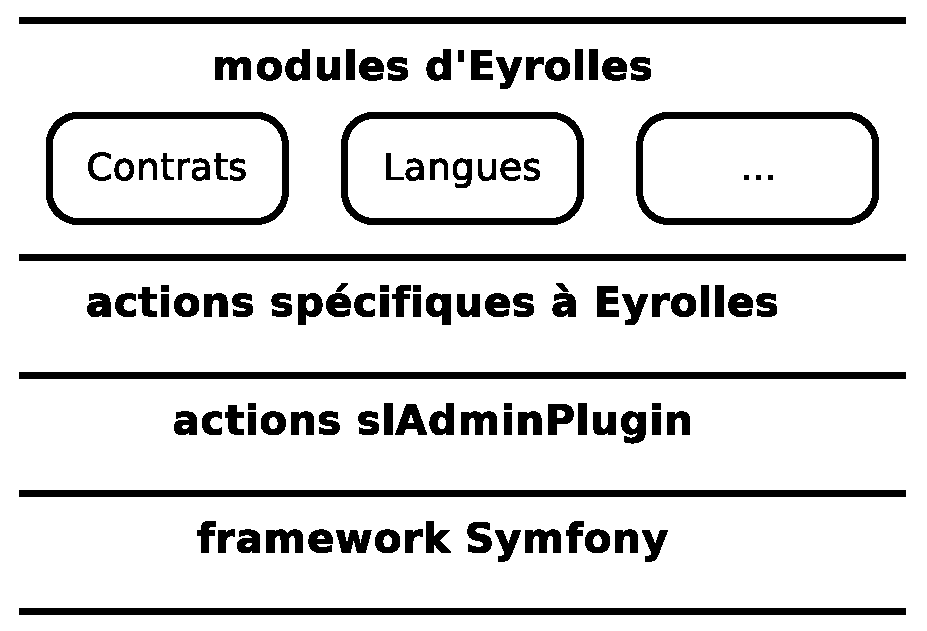
\includegraphics[scale=0.4]{eyrolles_modules_couches}
	\caption{Organisation des modules du \alotdeux\ d'\aey}
	\label{figure:eyrolles_modules_couches}
\end{figure}

\subsection{Modélisation des \awss}

La fonctionnalité des \awss\ annoncée en partie~\ref{section:eyrolles_fct} se résume à permettre à l'application développée, le \alotdeux, de communiquer avec la partie de l'\aintranet\ déjà existante, le \alotun.

Techniquement, un \aws\ est une interface (\aapi) accessible via un réseau et qui permet d'exécuter des actions sur un système distant. Dans le cas d'\aey, c'est le \alotdeux\ qui utilise l'interface du \alotun\footnote{Les \awss\ du \alotun\ sont développés en interne chez \aey.}, et jamais l'inverse. Les \awss\ du \alotdeux\ consistent alors à envoyer des données dans le bon format aux \awss\ du \alotun, et éventuellement de recevoir une réponse. Les données sont échangées via le protocole \ahttp, et le format de données utilisé est le \ajson\footnote{JSON (JavaScript Object Notation) est un format de données textuel permettant de représenter de l'information structurée.\\Exemple : \texttt{\{"auteur": \{"id": "1", "nom": "Jean Dupont"\}\}}}. La figure~\ref{figure:eyrolles_webservices_echange} illustre la façon dont les lots indépendants de l'\aintranet\ d'\aey\ communiquent.

\begin{figure}
	\centering
	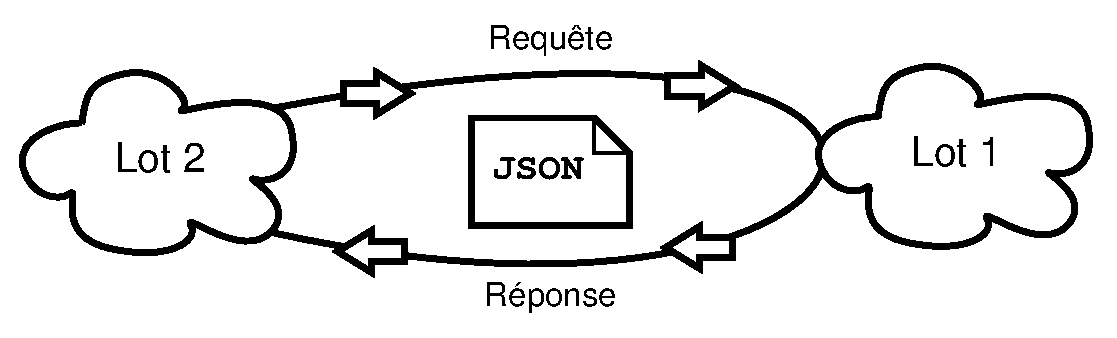
\includegraphics[scale=0.6]{eyrolles_webservices_echange}
	\caption{Principe de communication via \aws\ entre le \alotun\ et le \alotdeux\ d'\aey}
	\label{figure:eyrolles_webservices_echange}
\end{figure}

Les \awss\ à développer sur le \alotdeux\ sont les suivants :

\begin{itemize}
	\item le \aws\ des auteurs (initialisation et mise à jour) ;
	\item le \aws\ des collections (initialisation et mise à jour) ;
	\item le \aws\ des thématiques (initialisation) ;
	\item le \aws\ de demande de référencement ;
	\item le \aws\ de mise à jour des statuts de projets ;
	\item le \aws\ de mise à jour des informations commerciales des projets.
\end{itemize}

Tous ces types de \aws\ diffèrent en fait par l'adresse à laquelle ils doivent envoyer leur requête et par les paramètres qu'ils doivent fournir. Le processus d'échange de données avec le \alotun, quant à lui, est commun à tous. Le système à implémenter doit donc être modélisé, afin d'éviter d'écrire du code redondant et de faciliter une maintenance ultérieure. Cette étape de modélisation est une tâche clé du travail d'ingénieur, dans le sens où elle est nécessaire pour anticiper une évolution pérenne d'un système.

Le diagramme \auml\ de la figure~\ref{figure:eyrolles_webservices_uml} reprend la modélisation qui a été effectivement choisie.

\begin{figure}
	\centering
	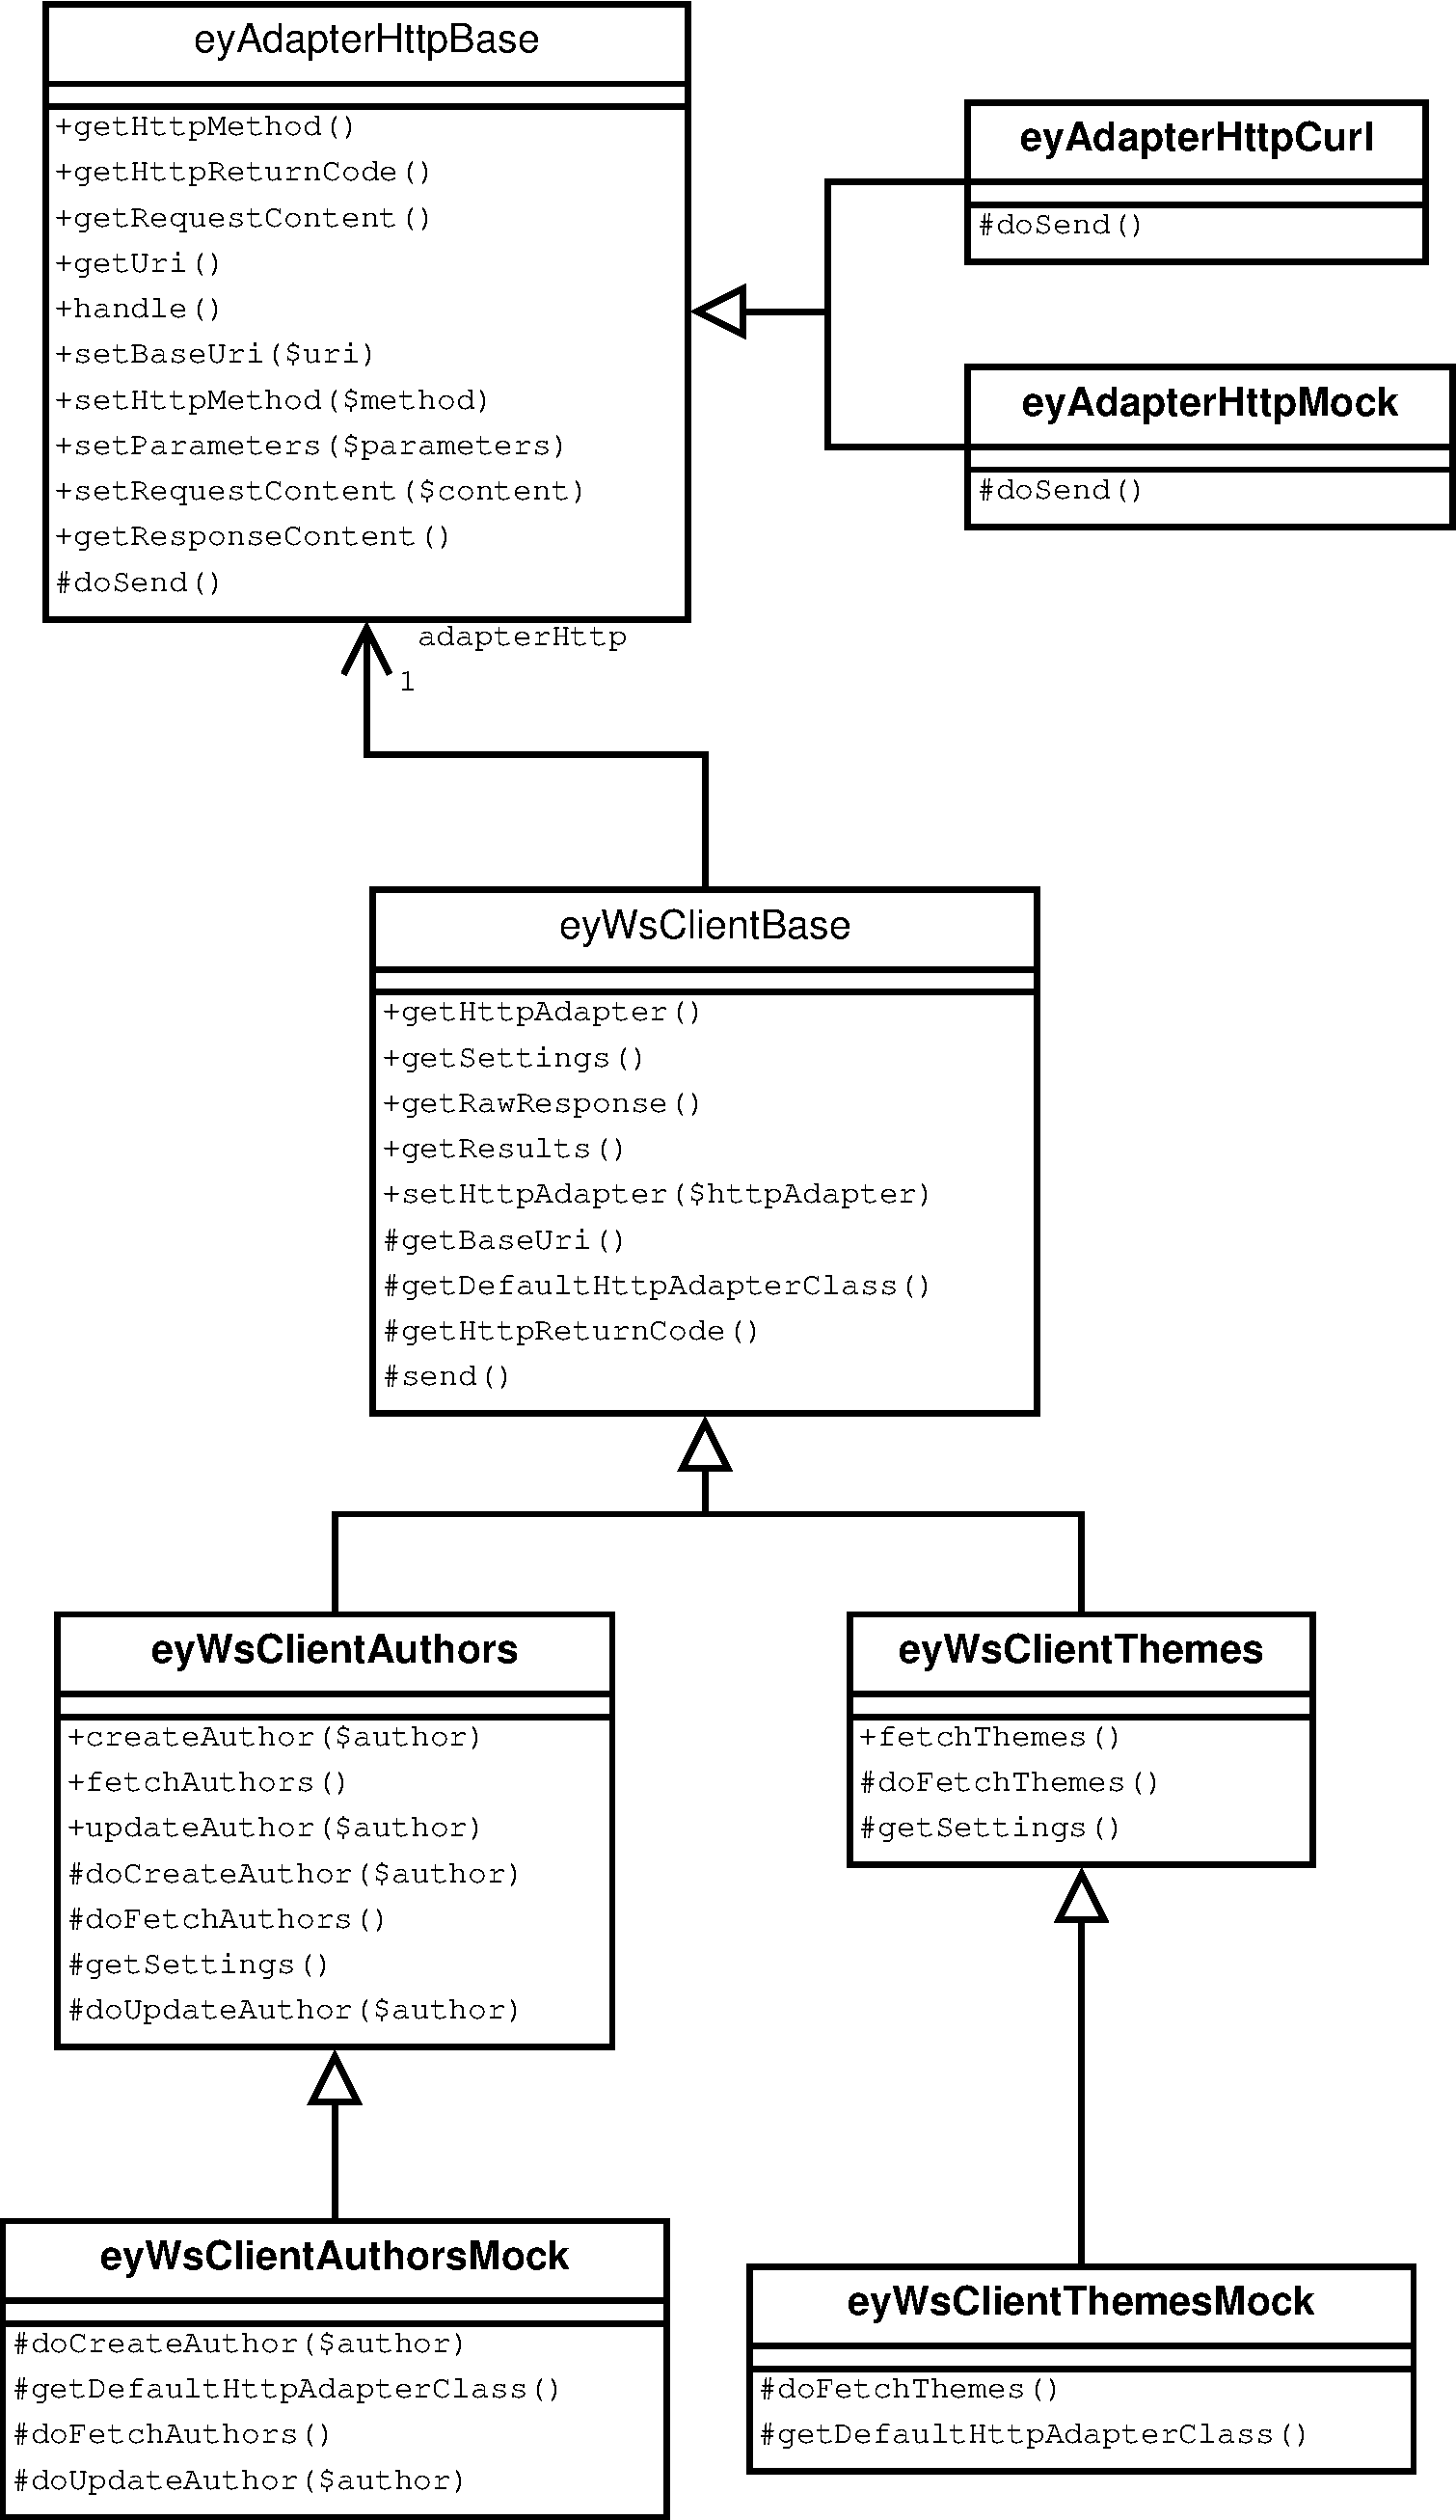
\includegraphics[scale=0.4]{eyrolles_webservices_uml}
	\caption{Modélisation des classes de \aws}
	\label{figure:eyrolles_webservices_uml}
\end{figure}

En effet, l'ensemble du code concernant la procédure de communication a été factorisé dans une classe \texttt{eyWsClientBase}. Les classes qui héritent de celle-ci, comme \texttt{eyWsClientAuthors} ou \texttt{eyWsClientThemes}, représentent les différents types de \aws. Au final, ces classes filles ne contiennent que les méthodes consistant à définir quels paramètres doivent être envoyés dans la requête, ou encore comment retourner la réponse à l'application.

Par ailleurs, l'implémentation de la liaison \ahttp\ a été isolée des classes de \aws\ : la classe abstraite \texttt{eyAdapterHttpBase} regroupe l'ensemble des méthodes permettant de stocker la méthode \ahttp\ à utiliser, les paramètres à envoyer ou encore l'adresse distante à consulter. Le contact effectif du \aws\ distant s'effectue dans la méthode \texttt{doSend()} surchargée dans les classes filles, telles que \texttt{eyAdapterHttpCurl} par exemple. Chaque classe \texttt{eyWsClient*} fait alors appel à une classe \texttt{eyAdapterHttp*} qui va se charger d'envoyer les données via le protocole \ahttp.

L'intérêt d'avoir différentes classes héritant de \texttt{eyAdapterHttpBase} permet de pouvoir implémenter de différentes façons l'appel au \aws\ distant. En effet, sur \aey, ce sont les fonctions de l'extension \acurl\footnote{La libraire \acurl\ donne la possibilité de récupérer, de créer ou encore de modifier le contenu d'une ressource accessible par le réseau, et supporte nottamment le protocole \ahttp.} de \aphp\ qui sont utilisées. En imaginant que l'\aintranet\ d'\aey\ soit déplacé sur un serveur sur lequel l'extension n'est pas installée, il serait très facile de réécrire une classe alternative, comme \texttt{eyAdapterHttpStream} qui utiliserait les fonctions \texttt{stream} disponibles en natif.

En outre, quand un développeur teste l'application du \alotdeux\ avec des données factices, il n'est pas concevable que celles-ci soient effectivement envoyées au \alotun\ pour le mettre à jour, au risque de corrompre l'intégrité des données de production. Il est donc nécessaire de prévoir une façon de simuler l'appel à un \aws.

Par exemple, dans le cas du \aws\ des auteurs, une classe \texttt{ey\-Ws\-Client\-Authors\-Mock} hérite de la classe \texttt{eyWsClientAuthors}. Entre autres, elle redéfinit la méthode sensée envoyer une requête de mise à jour d'un auteur au \alotun\ et ne fait rien à la place. Il est ainsi aisé de redéfinir des comportements initiaux, une fois que le problème a été modélisé en faisant appel aux grands principes de la programmation orientée objet.


\subsection{Écriture de tests}

Le projet \aey\ n'échappe pas à la règle : comme ses pairs, il est lui aussi soumis, via \asismo, au processus d'intégration continue décrit dans la partie~\ref{section:sismo}.

Le \afm\ \asf\ supporte deux types de tests : les tests unitaires et les tests fonctionnels.


\subsubsection{Tests unitaires}

\begin{quote}
Le test unitaire est un procédé permettant de s'assurer du fonctionnement correct d'une partie déterminée d'un logiciel ou d'une portion d'un programme.\cite{unit}
\end{quote}

Avec \asf, la bonne pratique consiste à tester les méthodes des classes de modèle et des classes utilitaires, indépendamment du reste de l'application. En effet, si à un moment ou un autre un des développeurs modifie le comportement de l'une des méthodes clés testées, les tests unitaires concernés deviendront potentiellement invalides.

Deux cas sont alors possibles : soit le nouveau comportement est désiré, soit au contraire c'est une erreur. Dans le premier cas, les tests unitaires ainsi que les parties de l'application qui utilisent leurs spécifications doivent être modifiés en conséquence. Dans le second, le comportement doit revenir dans son état précédent alors que les tests restent intacts. Dans chaque situation, le but est de ramener la suite de tests vers son état valide. Ainsi, l'écriture de tests unitaires est une bonne façon de s'assurer que toute modification de code testé sera suivie d'une vérification.

Une façon de tester unitairement une méthode consiste à l'appeler plusieurs fois, avec des paramètres ou un contexte différent. On vérifie alors si les valeurs retournées sont bien celles attendues, si une exception est propagée, si le contexte est de le bon état, etc.

Dans \asf, les tests unitaires sont effectués à l'aide du \afm\ de test unitaire \alime, développé pour \asf. Sur le projet \aey, ils ont été écrits tout au long du cycle de développement. Par souci de pragmatisme, seules les méthodes relativement importantes sont testées : il s'agit de ne pas perdre de temps avec les méthodes évidentes, ce qui reviendrait à tester les fonctionnalités de \asf\ elles-mêmes déjà unitairement testées de leur côté.

Par ailleurs, certaines fonctionnalités du projet à la logique poussée ont été développée en utilisant la méthode Test driven development (TDD), soit le développement 

Au delà de prévenir les régressions sur le projet, l'écriture de tests unitaires a permis de mettre à l'épreuve rapidement chaque mé


\subsubsection{Tests fonctionnels}

TODO


\subsection{Processus de mise en production}

TODO

\subsection{Bilan}

TODO


\section{Mini-développements}


\section{Participation à la vie de l'entreprise}

Tout au long de mon stage chez \asl, j'ai eu l'occasion d'assister à quelques formations internes qui concernaient les membres de l'équipe de développement. Les thèmes abordés étaient les suivants :

\begin{description}
	\item[\apsql] un fameux système de gestion de base de données relationnelle et objet libre ;
	\item[\aswift] le nouveau système d'envoi d'\aemails\ intégré à \asf ;
	\item[\atwig] un moteur de \atemplate\ libre développé par \apotencier ;
	\item[\asvnmerge] un outil pour \asvn ;
	\item[\amagento] une plateforme libre d'\aecommerce.
\end{description}

J'ai eu également l'opportunité de participer au bilan~2009 de \asensio, durant lequel ont été dévoilés les premiers chiffres de l'année et a été annoncée la ligne directrice pour 2010. Enfin, j'ai pu prendre part à des réunions concernant les méthodologies de l'entreprise, dont le but était de critiquer les processus de travail afin de les améliorer.


\chapter{Conclusion}

\section{Compétences acquises}

\begin{itemize}
\item commits atomiques
\end{itemize}


\newpage

%\bibliographystyle{plain}
%\addcontentsline{toc}{chapter}{Bibliographie}
%\nocite{*}
%\bibliography{biblio}
%\newpage

\appendix

\chapter{Captures d'écran}

\begin{figure}[h]
	\centering
	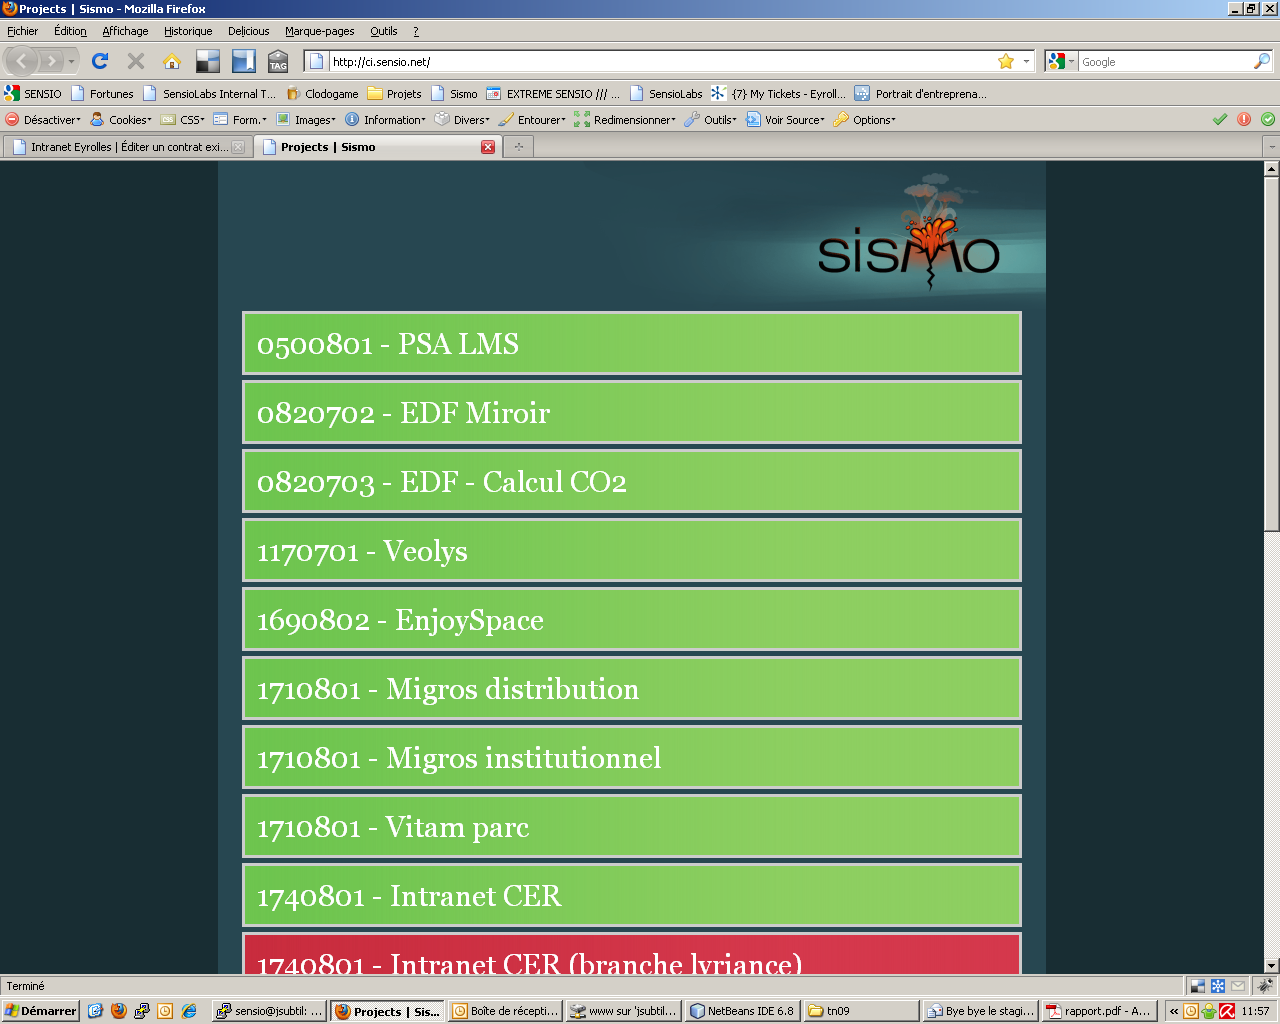
\includegraphics[width=10cm]{outils_sismo_screenshots_liste}
	\caption{Capture d'écran de la liste des projets sur \asismo}
	\label{figure:outils_sismo_screenshots_liste}
\end{figure}

\begin{figure}[h]
	\centering
	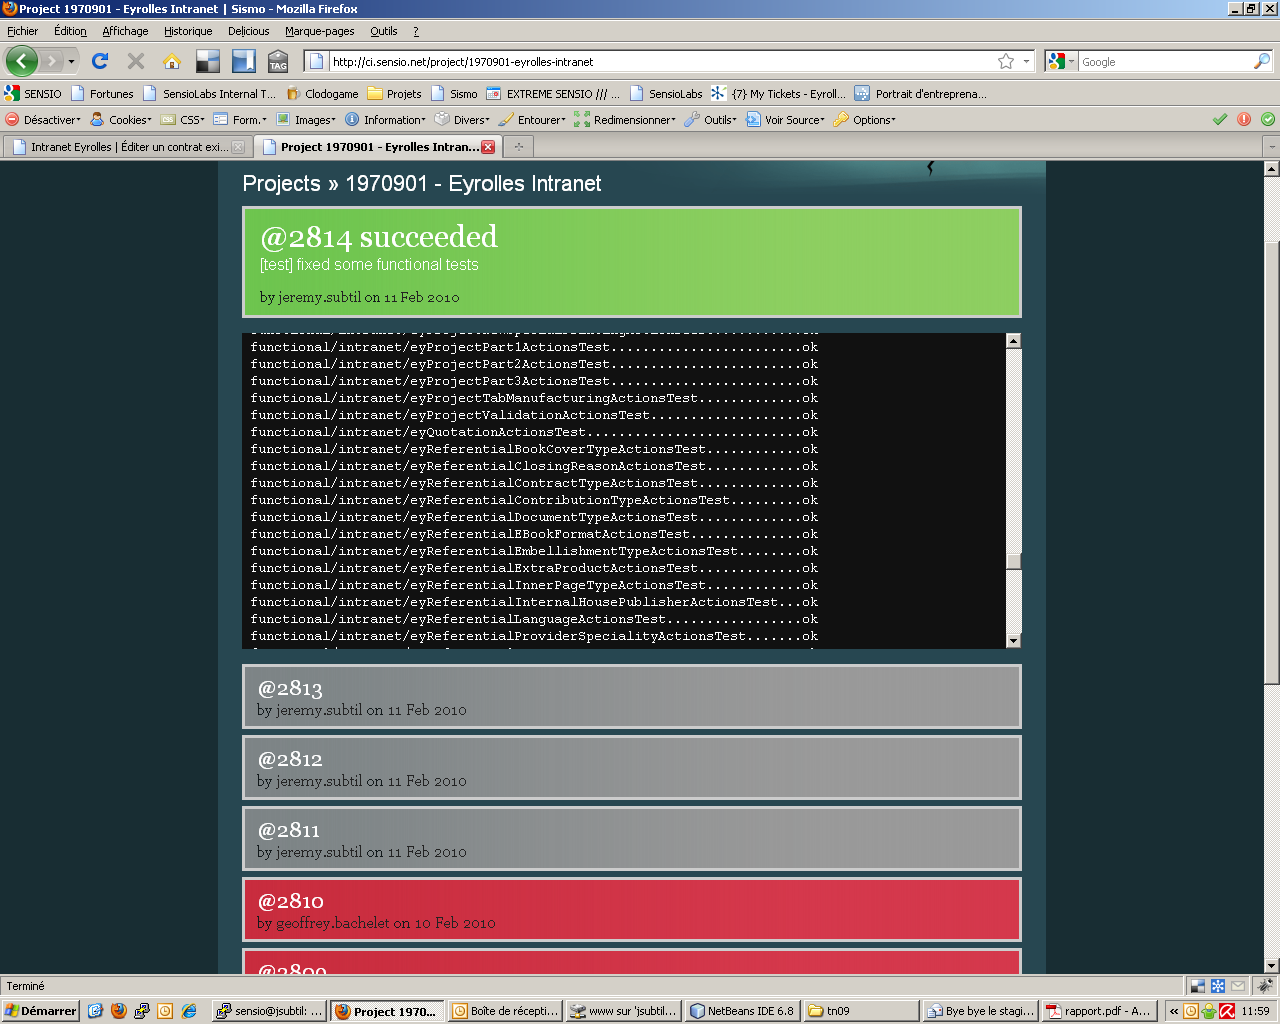
\includegraphics[width=10cm]{outils_sismo_screenshots_projet}
	\caption{Capture d'écran d'une fiche projet sur \asismo}
	\label{figure:outils_sismo_screenshots_projet}
\end{figure}

\begin{figure}[h]
	\centering
	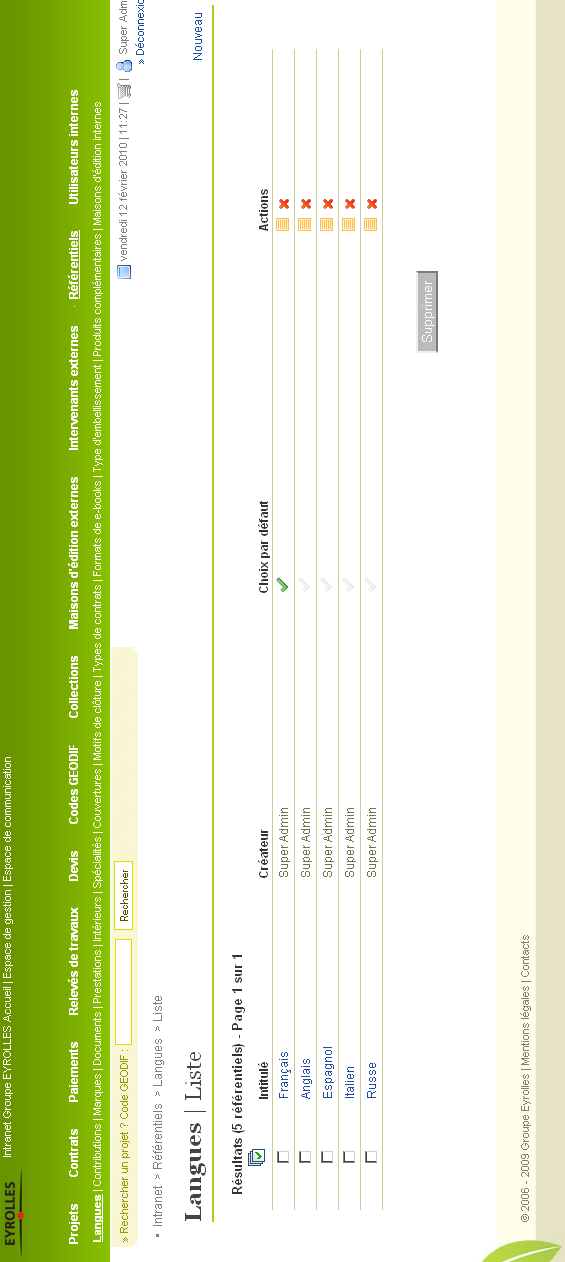
\includegraphics[width=10cm]{eyrolles_screenshots_language-list}
	\caption{Capture d'écran de la liste langues dans le \alotdeux\ de l'\aintranet\ d'\aey}
	\label{figure:eyrolles_screenshots_language-list}
\end{figure}

\begin{figure}[h]
	\centering
	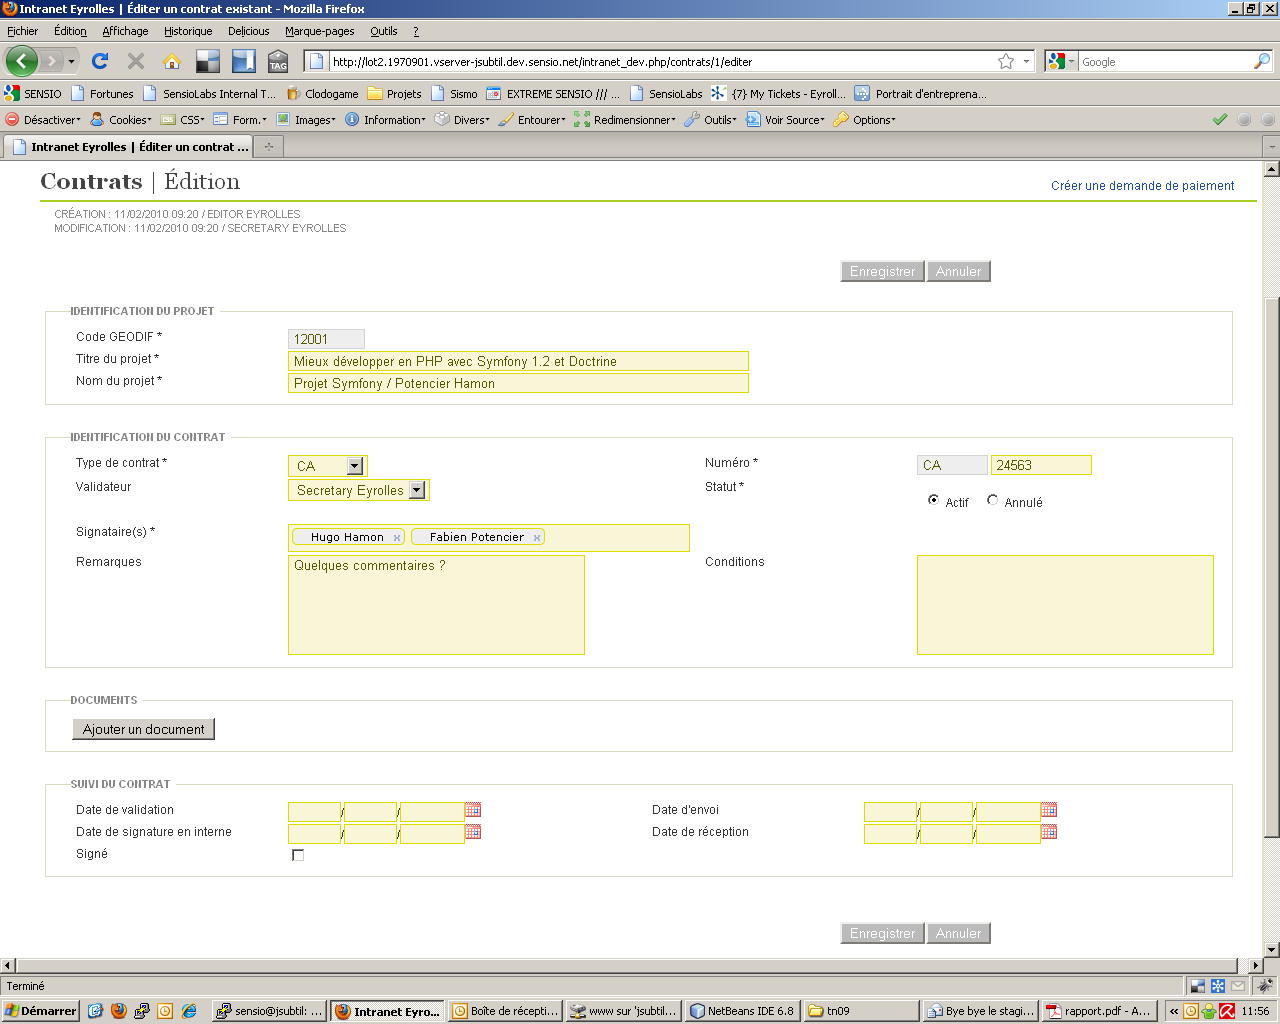
\includegraphics[width=10cm]{eyrolles_screenshots_contract-edit}
	\caption{Capture d'écran de l'édition d'un contrat dans le \alotdeux\ de l'\aintranet\ d'\aey}
	\label{figure:eyrolles_screenshots_contract-edit}
\end{figure}

\begin{figure}[h]
	\centering
	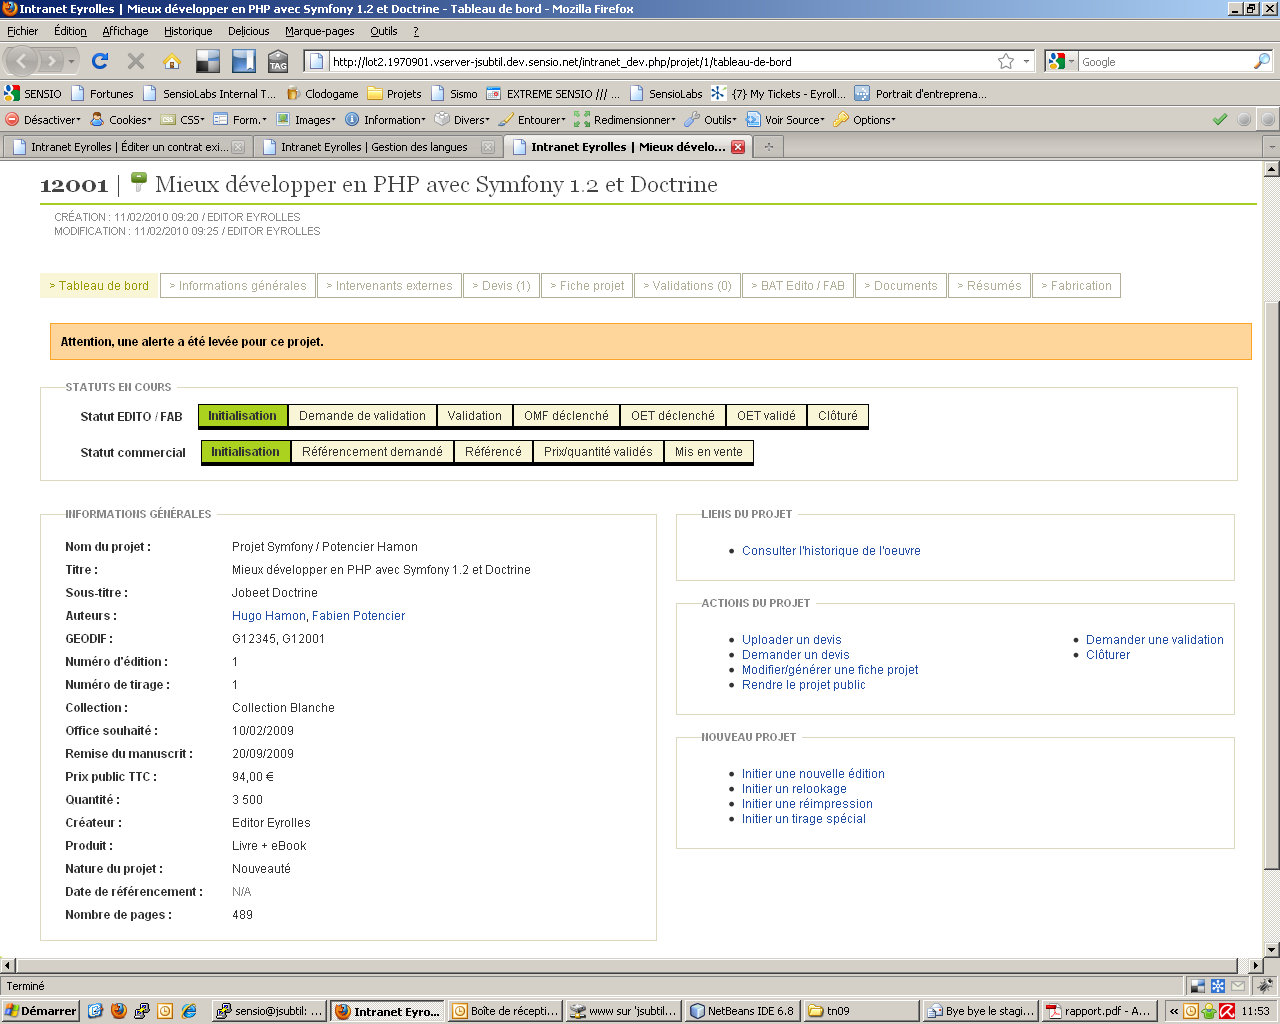
\includegraphics[width=10cm]{eyrolles_screenshots_project-board}
	\caption{Capture d'écran du tableau de bord d'un projet dans le \alotdeux\ de l'\aintranet\ d'\aey}
	\label{figure:eyrolles_screenshots_project-board}
\end{figure}


\end{document}
